\section{Dimensionality Reduction, PCA}
\begin{itemize}
	\item Before we dive into this, we should talk a bit about unsupervised learning.
		So far, with supervised learning, we have data in the form of \( \{(x_i,
		y_i)\} \) where you have an \( x \) and also an associated value \( y \). In
		unsupervised learning, you only have \( \{x_i\} \), with no associated
		outputs.
\end{itemize}

\subsection{Dimensionality Reduction}
\begin{itemize}
	\item What does it even mean to reduce the dimension? Suppose you have
		3-dimensional data that lives a spiral:
		\begin{center}
			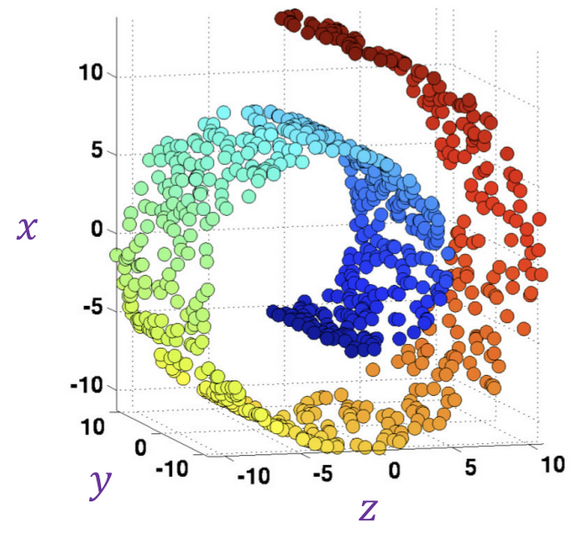
\includegraphics[scale=0.5]{images/lec12-1.png}
		\end{center}
		Could you determine the dataset by using 2 coordinates? The answer looks like
		yes. 
	\item In general, this is also the case. The manifold hypothesis says that high
		dimensional data tends to lie in the vicinity of a low dimensional manifold,
		basically motivating the fact that we can reduce dimensions without losing
		information. 

		\comment{A manifold for us is basically just a space that locally feels like 
			a euclidean space. For us, this manifold is going to be the lower 
		dimensional part of the observational space in which our data will lie.}

		The operation of dimensionality reduction is called an \textit{embedding}.  
\end{itemize}

\subsection{Principal Component Analysis (PCA)}
\begin{itemize}
	\item The trick with dimensionality reduction is to pick a clever basis in which
		we can still faithfully represent all images, in a lower dimension. 
	\item As an example, imagine first that your data lies in 2 dimensions. To reduce
		dimension, we basically want to look for the direction along which we retain
		the most information if you project the data onto it. To determine the
		direction, you find the direction which minimizes the \textit{reconstruction
		loss}.

		It turns out, the direction is the one which maximizes the variance of the
		data. Intuitively, this is because projecting onto a high variance makes the
		region in which the data lies larger. 
	\item The idea of PCA is to recursively apply this method -- we pick the first
		direction, then we pick the second direction which maximizes variance (which
		is orthogonal to the first one), and so on. The maximum number of basis
		vectors is obviously the dimension of the original space, but obviously you
		don't want to do that because your whole goal is dimensionality reduction.  
	\item As an aside, there is a probabilistic PCA that uses MLE which derives the
		exact same result. 
	\item To do PCA, you take the spectral decomposition (aka eigendecomposition) 
		of the covariance matrix \( A = QDQ^{\top} \), to find the principal
		components. 
	\item As an overview, this is what we do:
		\begin{itemize}
			\item Start with a data matrix \( X \in \R^{n \times d} \), center the
				data (zero mean) and then construct \( X^{\top} X \), 
				which is now symmetric. 
			\item Apply spectral theorem, so we get \( X^{\top} X = QDQ^{\top} \) and
				take the top \( k \) eigenvectors to pick off the \( k \) directions
				you want. 

				\question{How are the eigenvalues related related to the variance?} 
			\item Now, you approximate the new matrix with the best rank \( k \)
				matrix. You can do this by projecting all the original points \( X \)
				onto this new subspace, to make \( \overline X_k = \overline X Q_k\).
				Here, \( Q_k \) is the matrix of the first \( k \) eigenvectors. 
		\end{itemize}
	\item To visually see what information you lost, you can reconstruct the data
		using \( \overline X_\text{reconstructed} = \overline X_k Q_k^{\top} = 
		\overline X Q_k	Q_k^{\top}\). You can then compute the reconstruction loss,
		which is given by:
		\[
			\|\overline X_\text{recon-k} - \overline X\|_F
		\]
		It can also be proven via the Eckart-Young theorem that PCA gives a minimal
		reconstruction loss. 
	\item So what do you do pick \( k \)? You can compute the cumulative variance you
		keep from picking the first \( k \), and decide based on that.  
\end{itemize}

\subsection{Singular Value Decomposition (SVD)}
\begin{itemize}
	\item For any matrix \( M \), we can decompose it into \( M = U \Sigma V \),
		where \( U, V \) are square matrices, and \( \Sigma \) is a "diagonal"
		rectangular matrix. \( U \), \( V \) have the property that they're both
		orthonormal, so \( U U^{\top} = VV^{\top} = I \). 
	\item If you have very high dimensional images, then spectral decomposition would
		take an extremely long time because it's cubic in that dimension. SVD on the
		other hand is linear in the higher dimension and quadratic in the smaller, so
		it's computationally cheaper. 
	\item The column vectors in \( U \) are the eigenvectors of \( M M^{\top} \),
		which is exactly what we wanted to find in PCA anyways! So, you get both
		spectral decompositions at once, for \( M^{\top}M \) and also \( M M^{\top}
		\). 
	\item The eigenvalues are the same, and are given by \( \lambda_i = \Sigma_{ii}^2
		\), where \( \Sigma_{ii} \) lies on the diagonal of the \( \Sigma \) matrix. 
\end{itemize}
